\documentclass[1p]{elsarticle_modified}
%\bibliographystyle{elsarticle-num}

%\usepackage[colorlinks]{hyperref}
%\usepackage{abbrmath_seonhwa} %\Abb, \Ascr, \Acal ,\Abf, \Afrak
\usepackage{amsfonts}
\usepackage{amssymb}
\usepackage{amsmath}
\usepackage{amsthm}
\usepackage{scalefnt}
\usepackage{amsbsy}
\usepackage{kotex}
\usepackage{caption}
\usepackage{subfig}
\usepackage{color}
\usepackage{graphicx}
\usepackage{xcolor} %% white, black, red, green, blue, cyan, magenta, yellow
\usepackage{float}
\usepackage{setspace}
\usepackage{hyperref}

\usepackage{tikz}
\usetikzlibrary{arrows}

\usepackage{multirow}
\usepackage{array} % fixed length table
\usepackage{hhline}

%%%%%%%%%%%%%%%%%%%%%
\makeatletter
\renewcommand*\env@matrix[1][\arraystretch]{%
	\edef\arraystretch{#1}%
	\hskip -\arraycolsep
	\let\@ifnextchar\new@ifnextchar
	\array{*\c@MaxMatrixCols c}}
\makeatother %https://tex.stackexchange.com/questions/14071/how-can-i-increase-the-line-spacing-in-a-matrix
%%%%%%%%%%%%%%%

\usepackage[normalem]{ulem}

\newcommand{\msout}[1]{\ifmmode\text{\sout{\ensuremath{#1}}}\else\sout{#1}\fi}
%SOURCE: \msout is \stkout macro in https://tex.stackexchange.com/questions/20609/strikeout-in-math-mode

\newcommand{\cancel}[1]{
	\ifmmode
	{\color{red}\msout{#1}}
	\else
	{\color{red}\sout{#1}}
	\fi
}

\newcommand{\add}[1]{
	{\color{blue}\uwave{#1}}
}

\newcommand{\replace}[2]{
	\ifmmode
	{\color{red}\msout{#1}}{\color{blue}\uwave{#2}}
	\else
	{\color{red}\sout{#1}}{\color{blue}\uwave{#2}}
	\fi
}

\newcommand{\Sol}{\mathcal{S}} %segment
\newcommand{\D}{D} %diagram
\newcommand{\A}{\mathcal{A}} %arc


%%%%%%%%%%%%%%%%%%%%%%%%%%%%%5 test

\def\sl{\operatorname{\textup{SL}}(2,\Cbb)}
\def\psl{\operatorname{\textup{PSL}}(2,\Cbb)}
\def\quan{\mkern 1mu \triangleright \mkern 1mu}

\theoremstyle{definition}
\newtheorem{thm}{Theorem}[section]
\newtheorem{prop}[thm]{Proposition}
\newtheorem{lem}[thm]{Lemma}
\newtheorem{ques}[thm]{Question}
\newtheorem{cor}[thm]{Corollary}
\newtheorem{defn}[thm]{Definition}
\newtheorem{exam}[thm]{Example}
\newtheorem{rmk}[thm]{Remark}
\newtheorem{alg}[thm]{Algorithm}

\newcommand{\I}{\sqrt{-1}}
\begin{document}

%\begin{frontmatter}
%
%\title{Boundary parabolic representations of knots up to 8 crossings}
%
%%% Group authors per affiliation:
%\author{Yunhi Cho} 
%\address{Department of Mathematics, University of Seoul, Seoul, Korea}
%\ead{yhcho@uos.ac.kr}
%
%
%\author{Seonhwa Kim} %\fnref{s_kim}}
%\address{Center for Geometry and Physics, Institute for Basic Science, Pohang, 37673, Korea}
%\ead{ryeona17@ibs.re.kr}
%
%\author{Hyuk Kim}
%\address{Department of Mathematical Sciences, Seoul National University, Seoul 08826, Korea}
%\ead{hyukkim@snu.ac.kr}
%
%\author{Seokbeom Yoon}
%\address{Department of Mathematical Sciences, Seoul National University, Seoul, 08826,  Korea}
%\ead{sbyoon15@snu.ac.kr}
%
%\begin{abstract}
%We find all boundary parabolic representation of knots up to 8 crossings.
%
%\end{abstract}
%\begin{keyword}
%    \MSC[2010] 57M25 
%\end{keyword}
%
%\end{frontmatter}

%\linenumbers
%\tableofcontents
%
\newcommand\colored[1]{\textcolor{white}{\rule[-0.35ex]{0.8em}{1.4ex}}\kern-0.8em\color{red} #1}%
%\newcommand\colored[1]{\textcolor{white}{ #1}\kern-2.17ex	\textcolor{white}{ #1}\kern-1.81ex	\textcolor{white}{ #1}\kern-2.15ex\color{red}#1	}

{\Large $\underline{11a_{70}~(K11a_{70})}$}

\setlength{\tabcolsep}{10pt}
\renewcommand{\arraystretch}{1.6}
\vspace{1cm}\begin{tabular}{m{100pt}>{\centering\arraybackslash}m{274pt}}
\multirow{5}{120pt}{
	\centering
	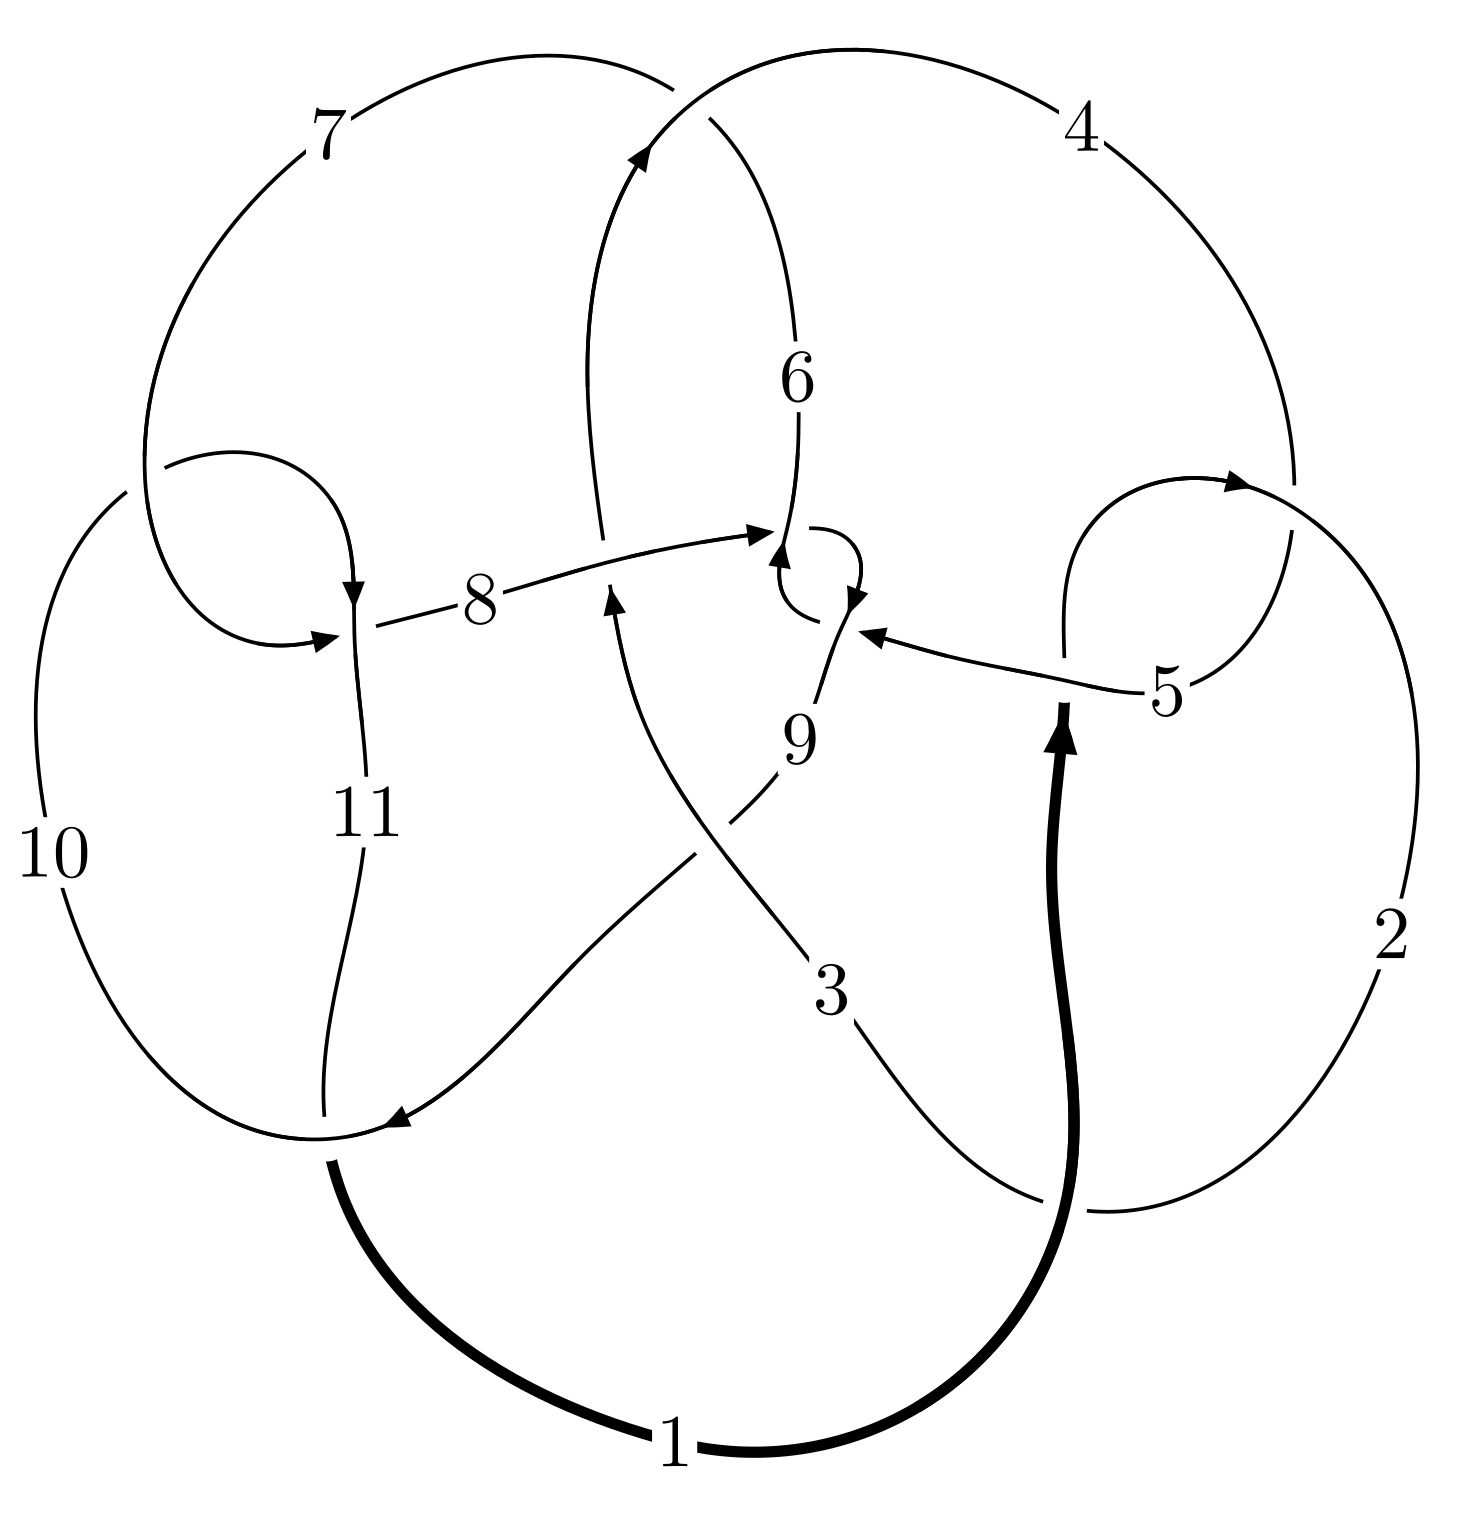
\includegraphics[width=112pt]{../../../GIT/diagram.site/Diagrams/png/319_11a_70.png}\\
\ \ \ A knot diagram\footnotemark}&
\allowdisplaybreaks
\textbf{Linearized knot diagam} \\
\cline{2-2}
 &
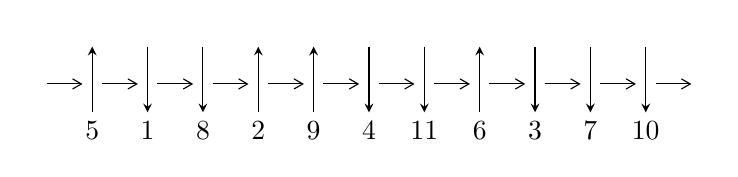
\begin{tikzpicture}[x=20pt, y=17pt]
	% nodes
	\node (C0) at (0, 0) {};
	\node (C1) at (1, 0) {};
	\node (C1U) at (1, +1) {};
	\node (C1D) at (1, -1) {5};

	\node (C2) at (2, 0) {};
	\node (C2U) at (2, +1) {};
	\node (C2D) at (2, -1) {1};

	\node (C3) at (3, 0) {};
	\node (C3U) at (3, +1) {};
	\node (C3D) at (3, -1) {8};

	\node (C4) at (4, 0) {};
	\node (C4U) at (4, +1) {};
	\node (C4D) at (4, -1) {2};

	\node (C5) at (5, 0) {};
	\node (C5U) at (5, +1) {};
	\node (C5D) at (5, -1) {9};

	\node (C6) at (6, 0) {};
	\node (C6U) at (6, +1) {};
	\node (C6D) at (6, -1) {4};

	\node (C7) at (7, 0) {};
	\node (C7U) at (7, +1) {};
	\node (C7D) at (7, -1) {11};

	\node (C8) at (8, 0) {};
	\node (C8U) at (8, +1) {};
	\node (C8D) at (8, -1) {6};

	\node (C9) at (9, 0) {};
	\node (C9U) at (9, +1) {};
	\node (C9D) at (9, -1) {3};

	\node (C10) at (10, 0) {};
	\node (C10U) at (10, +1) {};
	\node (C10D) at (10, -1) {7};

	\node (C11) at (11, 0) {};
	\node (C11U) at (11, +1) {};
	\node (C11D) at (11, -1) {10};
	\node (C12) at (12, 0) {};

	% arrows
	\draw[->,>={angle 60}]
	(C0) edge (C1) (C1) edge (C2) (C2) edge (C3) (C3) edge (C4) (C4) edge (C5) (C5) edge (C6) (C6) edge (C7) (C7) edge (C8) (C8) edge (C9) (C9) edge (C10) (C10) edge (C11) (C11) edge (C12) ;	\draw[->,>=stealth]
	(C1D) edge (C1U) (C2U) edge (C2D) (C3U) edge (C3D) (C4D) edge (C4U) (C5D) edge (C5U) (C6U) edge (C6D) (C7U) edge (C7D) (C8D) edge (C8U) (C9U) edge (C9D) (C10U) edge (C10D) (C11U) edge (C11D) ;
	\end{tikzpicture} \\
\hhline{~~} \\& 
\textbf{Solving Sequence} \\ \cline{2-2} 
 &
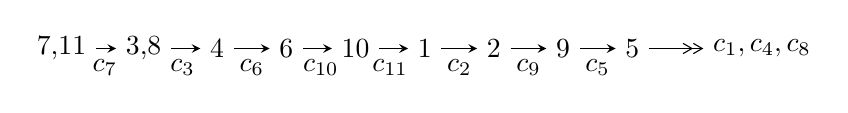
\begin{tikzpicture}[x=25pt, y=7pt]
	% node
	\node (A0) at (-1/8, 0) {7,11};
	\node (A1) at (17/16, 0) {3,8};
	\node (A2) at (17/8, 0) {4};
	\node (A3) at (25/8, 0) {6};
	\node (A4) at (33/8, 0) {10};
	\node (A5) at (41/8, 0) {1};
	\node (A6) at (49/8, 0) {2};
	\node (A7) at (57/8, 0) {9};
	\node (A8) at (65/8, 0) {5};
	\node (C1) at (1/2, -1) {$c_{7}$};
	\node (C2) at (13/8, -1) {$c_{3}$};
	\node (C3) at (21/8, -1) {$c_{6}$};
	\node (C4) at (29/8, -1) {$c_{10}$};
	\node (C5) at (37/8, -1) {$c_{11}$};
	\node (C6) at (45/8, -1) {$c_{2}$};
	\node (C7) at (53/8, -1) {$c_{9}$};
	\node (C8) at (61/8, -1) {$c_{5}$};
	\node (A9) at (10, 0) {$c_{1},c_{4},c_{8}$};

	% edge
	\draw[->,>=stealth]	
	(A0) edge (A1) (A1) edge (A2) (A2) edge (A3) (A3) edge (A4) (A4) edge (A5) (A5) edge (A6) (A6) edge (A7) (A7) edge (A8) ;
	\draw[->>,>={angle 60}]	
	(A8) edge (A9);
\end{tikzpicture} \\ 

\end{tabular} \\

\footnotetext{
The image of knot diagram is generated by the software ``\textbf{Draw programme}" developed by Andrew Bartholomew(\url{http://www.layer8.co.uk/maths/draw/index.htm\#Running-draw}), where we modified some parts for our purpose(\url{https://github.com/CATsTAILs/LinksPainter}).
}\phantom \\ \newline 
\centering \textbf{Ideals for irreducible components\footnotemark of $X_{\text{par}}$} 
 
\begin{align*}
I^u_{1}&=\langle 
-1.79690\times10^{82} u^{74}+7.20239\times10^{82} u^{73}+\cdots+6.04541\times10^{81} b-1.44668\times10^{82},\\
\phantom{I^u_{1}}&\phantom{= \langle  }-3.67725\times10^{81} u^{74}+1.14897\times10^{82} u^{73}+\cdots+6.04541\times10^{81} a-2.36959\times10^{81},\;u^{75}-5 u^{74}+\cdots-5 u^2-1\rangle \\
\\
\end{align*}
\raggedright * 1 irreducible components of $\dim_{\mathbb{C}}=0$, with total 75 representations.\\
\footnotetext{All coefficients of polynomials are rational numbers. But the coefficients are sometimes approximated in decimal forms when there is not enough margin.}
\newpage
\renewcommand{\arraystretch}{1}
\centering \section*{I. $I^u_{1}= \langle -1.80\times10^{82} u^{74}+7.20\times10^{82} u^{73}+\cdots+6.05\times10^{81} b-1.45\times10^{82},\;-3.68\times10^{81} u^{74}+1.15\times10^{82} u^{73}+\cdots+6.05\times10^{81} a-2.37\times10^{81},\;u^{75}-5 u^{74}+\cdots-5 u^2-1 \rangle$}
\flushleft \textbf{(i) Arc colorings}\\
\begin{tabular}{m{7pt} m{180pt} m{7pt} m{180pt} }
\flushright $a_{7}=$&$\begin{pmatrix}1\\0\end{pmatrix}$ \\
\flushright $a_{11}=$&$\begin{pmatrix}0\\u\end{pmatrix}$ \\
\flushright $a_{3}=$&$\begin{pmatrix}0.608272 u^{74}-1.90056 u^{73}+\cdots+1.36502 u+0.391965\\2.97234 u^{74}-11.9138 u^{73}+\cdots+0.909081 u+2.39302\end{pmatrix}$ \\
\flushright $a_{8}=$&$\begin{pmatrix}1\\u^2\end{pmatrix}$ \\
\flushright $a_{4}=$&$\begin{pmatrix}-0.754990 u^{74}+3.70568 u^{73}+\cdots+1.06421 u-0.860252\\2.28904 u^{74}-8.56988 u^{73}+\cdots-0.454181 u+1.18295\end{pmatrix}$ \\
\flushright $a_{6}=$&$\begin{pmatrix}0.735779 u^{74}-2.59000 u^{73}+\cdots-1.30849 u+3.10168\\2.66733 u^{74}-13.8183 u^{73}+\cdots-1.11611 u+0.260040\end{pmatrix}$ \\
\flushright $a_{10}=$&$\begin{pmatrix}u\\u\end{pmatrix}$ \\
\flushright $a_{1}=$&$\begin{pmatrix}- u^3\\- u^3+u\end{pmatrix}$ \\
\flushright $a_{2}=$&$\begin{pmatrix}-0.780163 u^{74}+4.52362 u^{73}+\cdots-0.0143966 u-1.25921\\2.96332 u^{74}-10.7355 u^{73}+\cdots-1.40070 u+1.40206\end{pmatrix}$ \\
\flushright $a_{9}=$&$\begin{pmatrix}-0.742503 u^{74}+5.31417 u^{73}+\cdots+6.61688 u+2.14994\\-0.526551 u^{74}+1.38417 u^{73}+\cdots-1.71851 u+1.60740\end{pmatrix}$ \\
\flushright $a_{5}=$&$\begin{pmatrix}1.78437 u^{74}-6.22270 u^{73}+\cdots+5.32082 u+2.42275\\2.41956 u^{74}-10.4227 u^{73}+\cdots+0.784371 u+2.69916\end{pmatrix}$\\ \flushright $a_{5}=$&$\begin{pmatrix}1.78437 u^{74}-6.22270 u^{73}+\cdots+5.32082 u+2.42275\\2.41956 u^{74}-10.4227 u^{73}+\cdots+0.784371 u+2.69916\end{pmatrix}$\\&\end{tabular}
\flushleft \textbf{(ii) Obstruction class $= -1$}\\~\\
\flushleft \textbf{(iii) Cusp Shapes $= -3.56995 u^{74}+12.8202 u^{73}+\cdots+11.6536 u-1.36638$}\\~\\
\newpage\renewcommand{\arraystretch}{1}
\flushleft \textbf{(iv) u-Polynomials at the component}\newline \\
\begin{tabular}{m{50pt}|m{274pt}}
Crossings & \hspace{64pt}u-Polynomials at each crossing \\
\hline $$\begin{aligned}c_{1},c_{4}\end{aligned}$$&$\begin{aligned}
&u^{75}+u^{74}+\cdots+16 u+1
\end{aligned}$\\
\hline $$\begin{aligned}c_{2}\end{aligned}$$&$\begin{aligned}
&u^{75}+31 u^{74}+\cdots+54 u-1
\end{aligned}$\\
\hline $$\begin{aligned}c_{3}\end{aligned}$$&$\begin{aligned}
&u^{75}+u^{74}+\cdots-10 u+1
\end{aligned}$\\
\hline $$\begin{aligned}c_{5},c_{8}\end{aligned}$$&$\begin{aligned}
&u^{75}+5 u^{74}+\cdots+5 u^2+1
\end{aligned}$\\
\hline $$\begin{aligned}c_{6}\end{aligned}$$&$\begin{aligned}
&u^{75}+u^{74}+\cdots+30 u-1
\end{aligned}$\\
\hline $$\begin{aligned}c_{7},c_{10}\end{aligned}$$&$\begin{aligned}
&u^{75}+5 u^{74}+\cdots+5 u^2+1
\end{aligned}$\\
\hline $$\begin{aligned}c_{9}\end{aligned}$$&$\begin{aligned}
&u^{75}+11 u^{74}+\cdots-828 u+297
\end{aligned}$\\
\hline $$\begin{aligned}c_{11}\end{aligned}$$&$\begin{aligned}
&u^{75}+29 u^{74}+\cdots-10 u+1
\end{aligned}$\\
\hline
\end{tabular}\\~\\
\newpage\renewcommand{\arraystretch}{1}
\flushleft \textbf{(v) Riley Polynomials at the component}\newline \\
\begin{tabular}{m{50pt}|m{274pt}}
Crossings & \hspace{64pt}Riley Polynomials at each crossing \\
\hline $$\begin{aligned}c_{1},c_{4}\end{aligned}$$&$\begin{aligned}
&y^{75}+31 y^{74}+\cdots+54 y-1
\end{aligned}$\\
\hline $$\begin{aligned}c_{2}\end{aligned}$$&$\begin{aligned}
&y^{75}+27 y^{74}+\cdots-1370 y-1
\end{aligned}$\\
\hline $$\begin{aligned}c_{3}\end{aligned}$$&$\begin{aligned}
&y^{75}-5 y^{74}+\cdots-18 y-1
\end{aligned}$\\
\hline $$\begin{aligned}c_{5},c_{8}\end{aligned}$$&$\begin{aligned}
&y^{75}+47 y^{74}+\cdots-10 y-1
\end{aligned}$\\
\hline $$\begin{aligned}c_{6}\end{aligned}$$&$\begin{aligned}
&y^{75}-121 y^{74}+\cdots+18 y-1
\end{aligned}$\\
\hline $$\begin{aligned}c_{7},c_{10}\end{aligned}$$&$\begin{aligned}
&y^{75}-29 y^{74}+\cdots-10 y-1
\end{aligned}$\\
\hline $$\begin{aligned}c_{9}\end{aligned}$$&$\begin{aligned}
&y^{75}+111 y^{74}+\cdots-4790502 y-88209
\end{aligned}$\\
\hline $$\begin{aligned}c_{11}\end{aligned}$$&$\begin{aligned}
&y^{75}+35 y^{74}+\cdots+118 y-1
\end{aligned}$\\
\hline
\end{tabular}\\~\\
\newpage\flushleft \textbf{(vi) Complex Volumes and Cusp Shapes}
$$\begin{array}{c|c|c}  
\text{Solutions to }I^u_{1}& \I (\text{vol} + \sqrt{-1}CS) & \text{Cusp shape}\\
 \hline 
\begin{aligned}
u &= \phantom{-}0.791299 + 0.626157 I \\
a &= -1.136250 - 0.194648 I \\
b &= -1.55325 - 0.23650 I\end{aligned}
 & \phantom{-}2.07598 + 0.79958 I & \phantom{-0.000000 } 0 \\ \hline\begin{aligned}
u &= \phantom{-}0.791299 - 0.626157 I \\
a &= -1.136250 + 0.194648 I \\
b &= -1.55325 + 0.23650 I\end{aligned}
 & \phantom{-}2.07598 - 0.79958 I & \phantom{-0.000000 } 0 \\ \hline\begin{aligned}
u &= \phantom{-}0.944435 + 0.356346 I \\
a &= -0.956319 - 0.093515 I \\
b &= -0.272280 - 1.297540 I\end{aligned}
 & -2.28865 - 1.17947 I & \phantom{-0.000000 } 0 \\ \hline\begin{aligned}
u &= \phantom{-}0.944435 - 0.356346 I \\
a &= -0.956319 + 0.093515 I \\
b &= -0.272280 + 1.297540 I\end{aligned}
 & -2.28865 + 1.17947 I & \phantom{-0.000000 } 0 \\ \hline\begin{aligned}
u &= -0.868230 + 0.530776 I \\
a &= -2.18646 + 8.50420 I \\
b &= \phantom{-}6.91289 + 6.22470 I\end{aligned}
 & -1.67548 + 0.05018 I & \phantom{-}33.6456 + 61.6621 I \\ \hline\begin{aligned}
u &= -0.868230 - 0.530776 I \\
a &= -2.18646 - 8.50420 I \\
b &= \phantom{-}6.91289 - 6.22470 I\end{aligned}
 & -1.67548 - 0.05018 I & \phantom{-}33.6456 - 61.6621 I \\ \hline\begin{aligned}
u &= -0.901384 + 0.490863 I \\
a &= -4.06027 - 6.10797 I \\
b &= -7.63991 - 0.14270 I\end{aligned}
 & -1.69112 + 4.00680 I & \phantom{-}36.1919 - 36.8000 I \\ \hline\begin{aligned}
u &= -0.901384 - 0.490863 I \\
a &= -4.06027 + 6.10797 I \\
b &= -7.63991 + 0.14270 I\end{aligned}
 & -1.69112 - 4.00680 I & \phantom{-}36.1919 + 36.8000 I \\ \hline\begin{aligned}
u &= \phantom{-}0.567539 + 0.856472 I \\
a &= -1.019940 + 0.924823 I \\
b &= -1.54560 - 0.33056 I\end{aligned}
 & \phantom{-}1.74716 + 5.71342 I & \phantom{-0.000000 } 0 \\ \hline\begin{aligned}
u &= \phantom{-}0.567539 - 0.856472 I \\
a &= -1.019940 - 0.924823 I \\
b &= -1.54560 + 0.33056 I\end{aligned}
 & \phantom{-}1.74716 - 5.71342 I & \phantom{-0.000000 } 0\\
 \hline 
 \end{array}$$\newpage$$\begin{array}{c|c|c}  
\text{Solutions to }I^u_{1}& \I (\text{vol} + \sqrt{-1}CS) & \text{Cusp shape}\\
 \hline 
\begin{aligned}
u &= \phantom{-}0.964338\phantom{ +0.000000I} \\
a &= \phantom{-}0.506841\phantom{ +0.000000I} \\
b &= -0.214290\phantom{ +0.000000I}\end{aligned}
 & -1.61136\phantom{ +0.000000I} & -5.58450\phantom{ +0.000000I} \\ \hline\begin{aligned}
u &= \phantom{-}0.765824 + 0.583007 I \\
a &= \phantom{-}0.303385 - 1.001710 I \\
b &= -0.196885 - 0.062255 I\end{aligned}
 & \phantom{-}1.55349 + 0.61348 I & \phantom{-0.000000 -}     -6
0. 10   + 1.237316 I \\ \hline\begin{aligned}
u &= \phantom{-}0.765824 - 0.583007 I \\
a &= \phantom{-}0.303385 + 1.001710 I \\
b &= -0.196885 + 0.062255 I\end{aligned}
 & \phantom{-}1.55349 - 0.61348 I & \phantom{-0.000000 }      -6
0. 10   - 1.237316 I \\ \hline\begin{aligned}
u &= -0.829499 + 0.630475 I \\
a &= \phantom{-}1.18877 + 1.25117 I \\
b &= \phantom{-}1.88802 + 0.62955 I\end{aligned}
 & \phantom{-}2.48636 + 2.32410 I & \phantom{-0.000000 } 0 \\ \hline\begin{aligned}
u &= -0.829499 - 0.630475 I \\
a &= \phantom{-}1.18877 - 1.25117 I \\
b &= \phantom{-}1.88802 - 0.62955 I\end{aligned}
 & \phantom{-}2.48636 - 2.32410 I & \phantom{-0.000000 } 0 \\ \hline\begin{aligned}
u &= -0.850863 + 0.627859 I \\
a &= \phantom{-}0.87390 + 1.79384 I \\
b &= \phantom{-}1.54353 + 0.99983 I\end{aligned}
 & \phantom{-}2.42103 + 2.60653 I & \phantom{-0.000000 } 0 \\ \hline\begin{aligned}
u &= -0.850863 - 0.627859 I \\
a &= \phantom{-}0.87390 - 1.79384 I \\
b &= \phantom{-}1.54353 - 0.99983 I\end{aligned}
 & \phantom{-}2.42103 - 2.60653 I & \phantom{-0.000000 } 0 \\ \hline\begin{aligned}
u &= \phantom{-}0.526837 + 0.922838 I \\
a &= \phantom{-}0.942081 - 1.033130 I \\
b &= \phantom{-}1.51134 + 0.47807 I\end{aligned}
 & -0.14883 + 11.48980 I & \phantom{-0.000000 } 0 \\ \hline\begin{aligned}
u &= \phantom{-}0.526837 - 0.922838 I \\
a &= \phantom{-}0.942081 + 1.033130 I \\
b &= \phantom{-}1.51134 - 0.47807 I\end{aligned}
 & -0.14883 - 11.48980 I & \phantom{-0.000000 } 0 \\ \hline\begin{aligned}
u &= -0.607991 + 0.890820 I \\
a &= \phantom{-}0.599024 + 0.851155 I \\
b &= \phantom{-}1.207750 - 0.075419 I\end{aligned}
 & \phantom{-}5.04527 - 0.07914 I & \phantom{-0.000000 } 0\\
 \hline 
 \end{array}$$\newpage$$\begin{array}{c|c|c}  
\text{Solutions to }I^u_{1}& \I (\text{vol} + \sqrt{-1}CS) & \text{Cusp shape}\\
 \hline 
\begin{aligned}
u &= -0.607991 - 0.890820 I \\
a &= \phantom{-}0.599024 - 0.851155 I \\
b &= \phantom{-}1.207750 + 0.075419 I\end{aligned}
 & \phantom{-}5.04527 + 0.07914 I & \phantom{-0.000000 } 0 \\ \hline\begin{aligned}
u &= \phantom{-}0.263630 + 0.876603 I \\
a &= -0.375992 - 0.459802 I \\
b &= -0.020158 - 0.411851 I\end{aligned}
 & \phantom{-}0.37773 - 1.86497 I & \phantom{-0.000000 -}0. + 5.71221 I \\ \hline\begin{aligned}
u &= \phantom{-}0.263630 - 0.876603 I \\
a &= -0.375992 + 0.459802 I \\
b &= -0.020158 + 0.411851 I\end{aligned}
 & \phantom{-}0.37773 + 1.86497 I & \phantom{-0.000000 } 0. - 5.71221 I \\ \hline\begin{aligned}
u &= \phantom{-}0.886820 + 0.625610 I \\
a &= -0.02345 + 1.84145 I \\
b &= -0.251662 + 1.256830 I\end{aligned}
 & \phantom{-}1.78310 - 5.71290 I & \phantom{-0.000000 } 0 \\ \hline\begin{aligned}
u &= \phantom{-}0.886820 - 0.625610 I \\
a &= -0.02345 - 1.84145 I \\
b &= -0.251662 - 1.256830 I\end{aligned}
 & \phantom{-}1.78310 + 5.71290 I & \phantom{-0.000000 } 0 \\ \hline\begin{aligned}
u &= \phantom{-}0.914521 + 0.590451 I \\
a &= \phantom{-}0.119679 + 0.166270 I \\
b &= \phantom{-}0.970439 - 0.336294 I\end{aligned}
 & \phantom{-}1.08449 - 5.28857 I & \phantom{-0.000000 } 0 \\ \hline\begin{aligned}
u &= \phantom{-}0.914521 - 0.590451 I \\
a &= \phantom{-}0.119679 - 0.166270 I \\
b &= \phantom{-}0.970439 + 0.336294 I\end{aligned}
 & \phantom{-}1.08449 + 5.28857 I & \phantom{-0.000000 } 0 \\ \hline\begin{aligned}
u &= \phantom{-}0.932597 + 0.568367 I \\
a &= \phantom{-}0.013751 + 1.184380 I \\
b &= -0.884923 + 0.749244 I\end{aligned}
 & -1.83222 - 2.08698 I & \phantom{-0.000000 } 0 \\ \hline\begin{aligned}
u &= \phantom{-}0.932597 - 0.568367 I \\
a &= \phantom{-}0.013751 - 1.184380 I \\
b &= -0.884923 - 0.749244 I\end{aligned}
 & -1.83222 + 2.08698 I & \phantom{-0.000000 } 0 \\ \hline\begin{aligned}
u &= -0.685629 + 0.592250 I \\
a &= -0.46109 - 2.41463 I \\
b &= -0.744705 - 1.183340 I\end{aligned}
 & -0.17676 - 3.45478 I & -1.78652 + 5.40342 I\\
 \hline 
 \end{array}$$\newpage$$\begin{array}{c|c|c}  
\text{Solutions to }I^u_{1}& \I (\text{vol} + \sqrt{-1}CS) & \text{Cusp shape}\\
 \hline 
\begin{aligned}
u &= -0.685629 - 0.592250 I \\
a &= -0.46109 + 2.41463 I \\
b &= -0.744705 + 1.183340 I\end{aligned}
 & -0.17676 + 3.45478 I & -1.78652 - 5.40342 I \\ \hline\begin{aligned}
u &= -0.515117 + 0.972701 I \\
a &= -0.527100 - 0.786396 I \\
b &= -0.995231 + 0.207120 I\end{aligned}
 & \phantom{-}4.01125 - 5.34018 I & \phantom{-0.000000 } 0 \\ \hline\begin{aligned}
u &= -0.515117 - 0.972701 I \\
a &= -0.527100 + 0.786396 I \\
b &= -0.995231 - 0.207120 I\end{aligned}
 & \phantom{-}4.01125 + 5.34018 I & \phantom{-0.000000 } 0 \\ \hline\begin{aligned}
u &= \phantom{-}0.445298 + 1.029250 I \\
a &= \phantom{-}0.435633 + 0.502400 I \\
b &= -0.295800 + 0.460901 I\end{aligned}
 & -0.63449 - 6.30730 I & \phantom{-0.000000 } 0 \\ \hline\begin{aligned}
u &= \phantom{-}0.445298 - 1.029250 I \\
a &= \phantom{-}0.435633 - 0.502400 I \\
b &= -0.295800 - 0.460901 I\end{aligned}
 & -0.63449 + 6.30730 I & \phantom{-0.000000 } 0 \\ \hline\begin{aligned}
u &= -0.955518 + 0.606406 I \\
a &= -1.62212 - 0.44289 I \\
b &= -2.45993 - 0.12029 I\end{aligned}
 & -0.99272 + 8.24278 I & \phantom{-0.000000 } 0 \\ \hline\begin{aligned}
u &= -0.955518 - 0.606406 I \\
a &= -1.62212 + 0.44289 I \\
b &= -2.45993 + 0.12029 I\end{aligned}
 & -0.99272 - 8.24278 I & \phantom{-0.000000 } 0 \\ \hline\begin{aligned}
u &= -1.128430 + 0.127839 I \\
a &= \phantom{-}0.202502 + 0.566795 I \\
b &= -0.874006 + 0.102629 I\end{aligned}
 & -9.45607 - 1.38465 I & \phantom{-0.000000 } 0 \\ \hline\begin{aligned}
u &= -1.128430 - 0.127839 I \\
a &= \phantom{-}0.202502 - 0.566795 I \\
b &= -0.874006 - 0.102629 I\end{aligned}
 & -9.45607 + 1.38465 I & \phantom{-0.000000 } 0 \\ \hline\begin{aligned}
u &= -1.145380 + 0.069325 I \\
a &= -0.679931 + 0.226099 I \\
b &= \phantom{-}0.221937 - 0.116509 I\end{aligned}
 & -4.70899 + 4.40582 I & \phantom{-0.000000 } 0\\
 \hline 
 \end{array}$$\newpage$$\begin{array}{c|c|c}  
\text{Solutions to }I^u_{1}& \I (\text{vol} + \sqrt{-1}CS) & \text{Cusp shape}\\
 \hline 
\begin{aligned}
u &= -1.145380 - 0.069325 I \\
a &= -0.679931 - 0.226099 I \\
b &= \phantom{-}0.221937 + 0.116509 I\end{aligned}
 & -4.70899 - 4.40582 I & \phantom{-0.000000 } 0 \\ \hline\begin{aligned}
u &= -1.043790 + 0.518555 I \\
a &= -1.00385 - 1.21751 I \\
b &= -1.48625 - 0.73116 I\end{aligned}
 & -2.22532 + 5.04203 I & \phantom{-0.000000 } 0 \\ \hline\begin{aligned}
u &= -1.043790 - 0.518555 I \\
a &= -1.00385 + 1.21751 I \\
b &= -1.48625 + 0.73116 I\end{aligned}
 & -2.22532 - 5.04203 I & \phantom{-0.000000 } 0 \\ \hline\begin{aligned}
u &= -0.742052 + 0.333850 I \\
a &= -0.49225 - 1.85952 I \\
b &= -1.13591 - 1.35983 I\end{aligned}
 & -0.76010 - 1.33278 I & -0.332802 + 0.983014 I \\ \hline\begin{aligned}
u &= -0.742052 - 0.333850 I \\
a &= -0.49225 + 1.85952 I \\
b &= -1.13591 + 1.35983 I\end{aligned}
 & -0.76010 + 1.33278 I & -0.332802 - 0.983014 I \\ \hline\begin{aligned}
u &= \phantom{-}0.795402 + 0.062224 I \\
a &= \phantom{-}1.62950 - 0.64233 I \\
b &= \phantom{-}1.09692 - 1.47817 I\end{aligned}
 & -3.90324 + 3.60828 I & -10.09775 - 4.41571 I \\ \hline\begin{aligned}
u &= \phantom{-}0.795402 - 0.062224 I \\
a &= \phantom{-}1.62950 + 0.64233 I \\
b &= \phantom{-}1.09692 + 1.47817 I\end{aligned}
 & -3.90324 - 3.60828 I & -10.09775 + 4.41571 I \\ \hline\begin{aligned}
u &= \phantom{-}1.055580 + 0.589429 I \\
a &= \phantom{-}0.72557 - 1.95839 I \\
b &= \phantom{-}1.62317 - 1.88315 I\end{aligned}
 & -6.54687 - 8.38886 I & \phantom{-0.000000 } 0 \\ \hline\begin{aligned}
u &= \phantom{-}1.055580 - 0.589429 I \\
a &= \phantom{-}0.72557 + 1.95839 I \\
b &= \phantom{-}1.62317 + 1.88315 I\end{aligned}
 & -6.54687 + 8.38886 I & \phantom{-0.000000 } 0 \\ \hline\begin{aligned}
u &= \phantom{-}0.397886 + 0.666525 I \\
a &= \phantom{-}1.49281 - 1.20707 I \\
b &= \phantom{-}1.199140 + 0.038507 I\end{aligned}
 & -4.74813 + 3.53322 I & -6.97223 - 3.25767 I\\
 \hline 
 \end{array}$$\newpage$$\begin{array}{c|c|c}  
\text{Solutions to }I^u_{1}& \I (\text{vol} + \sqrt{-1}CS) & \text{Cusp shape}\\
 \hline 
\begin{aligned}
u &= \phantom{-}0.397886 - 0.666525 I \\
a &= \phantom{-}1.49281 + 1.20707 I \\
b &= \phantom{-}1.199140 - 0.038507 I\end{aligned}
 & -4.74813 - 3.53322 I & -6.97223 + 3.25767 I \\ \hline\begin{aligned}
u &= \phantom{-}0.873447 + 0.870694 I \\
a &= \phantom{-}0.395339 + 0.623453 I \\
b &= -0.437516 + 0.908419 I\end{aligned}
 & -2.26517 - 1.56796 I & \phantom{-0.000000 } 0 \\ \hline\begin{aligned}
u &= \phantom{-}0.873447 - 0.870694 I \\
a &= \phantom{-}0.395339 - 0.623453 I \\
b &= -0.437516 - 0.908419 I\end{aligned}
 & -2.26517 + 1.56796 I & \phantom{-0.000000 } 0 \\ \hline\begin{aligned}
u &= -1.263390 + 0.059974 I \\
a &= \phantom{-}0.451522 - 0.021954 I \\
b &= -0.367243 + 0.519313 I\end{aligned}
 & -7.03947 + 9.35177 I & \phantom{-0.000000 } 0 \\ \hline\begin{aligned}
u &= -1.263390 - 0.059974 I \\
a &= \phantom{-}0.451522 + 0.021954 I \\
b &= -0.367243 - 0.519313 I\end{aligned}
 & -7.03947 - 9.35177 I & \phantom{-0.000000 } 0 \\ \hline\begin{aligned}
u &= \phantom{-}1.075430 + 0.686951 I \\
a &= -0.61564 + 1.81999 I \\
b &= -1.83957 + 1.40797 I\end{aligned}
 & \phantom{-}0.20150 - 11.45470 I & \phantom{-0.000000 } 0 \\ \hline\begin{aligned}
u &= \phantom{-}1.075430 - 0.686951 I \\
a &= -0.61564 - 1.81999 I \\
b &= -1.83957 - 1.40797 I\end{aligned}
 & \phantom{-}0.20150 + 11.45470 I & \phantom{-0.000000 } 0 \\ \hline\begin{aligned}
u &= -1.065960 + 0.707388 I \\
a &= \phantom{-}0.59448 + 1.33761 I \\
b &= \phantom{-}1.59308 + 0.92121 I\end{aligned}
 & \phantom{-}3.62731 + 5.97807 I & \phantom{-0.000000 } 0 \\ \hline\begin{aligned}
u &= -1.065960 - 0.707388 I \\
a &= \phantom{-}0.59448 - 1.33761 I \\
b &= \phantom{-}1.59308 - 0.92121 I\end{aligned}
 & \phantom{-}3.62731 - 5.97807 I & \phantom{-0.000000 } 0 \\ \hline\begin{aligned}
u &= \phantom{-}1.115700 + 0.695740 I \\
a &= \phantom{-}0.64039 - 1.78540 I \\
b &= \phantom{-}2.05325 - 1.45013 I\end{aligned}
 & -1.9580 - 17.4335 I & \phantom{-0.000000 } 0\\
 \hline 
 \end{array}$$\newpage$$\begin{array}{c|c|c}  
\text{Solutions to }I^u_{1}& \I (\text{vol} + \sqrt{-1}CS) & \text{Cusp shape}\\
 \hline 
\begin{aligned}
u &= \phantom{-}1.115700 - 0.695740 I \\
a &= \phantom{-}0.64039 + 1.78540 I \\
b &= \phantom{-}2.05325 + 1.45013 I\end{aligned}
 & -1.9580 + 17.4335 I & \phantom{-0.000000 } 0 \\ \hline\begin{aligned}
u &= \phantom{-}1.311660 + 0.204711 I \\
a &= -0.138053 + 0.165335 I \\
b &= \phantom{-}0.348061 + 0.219302 I\end{aligned}
 & -3.70859 - 2.85030 I & \phantom{-0.000000 } 0 \\ \hline\begin{aligned}
u &= \phantom{-}1.311660 - 0.204711 I \\
a &= -0.138053 - 0.165335 I \\
b &= \phantom{-}0.348061 - 0.219302 I\end{aligned}
 & -3.70859 + 2.85030 I & \phantom{-0.000000 } 0 \\ \hline\begin{aligned}
u &= -1.131880 + 0.708785 I \\
a &= -0.553642 - 1.238480 I \\
b &= -1.58959 - 1.00695 I\end{aligned}
 & \phantom{-}2.10726 + 11.44930 I & \phantom{-0.000000 } 0 \\ \hline\begin{aligned}
u &= -1.131880 - 0.708785 I \\
a &= -0.553642 + 1.238480 I \\
b &= -1.58959 + 1.00695 I\end{aligned}
 & \phantom{-}2.10726 - 11.44930 I & \phantom{-0.000000 } 0 \\ \hline\begin{aligned}
u &= \phantom{-}1.254070 + 0.541848 I \\
a &= \phantom{-}0.006977 - 0.440278 I \\
b &= -0.005491 - 0.633191 I\end{aligned}
 & -3.53974 + 0.15240 I & \phantom{-0.000000 } 0 \\ \hline\begin{aligned}
u &= \phantom{-}1.254070 - 0.541848 I \\
a &= \phantom{-}0.006977 + 0.440278 I \\
b &= -0.005491 + 0.633191 I\end{aligned}
 & -3.53974 - 0.15240 I & \phantom{-0.000000 } 0 \\ \hline\begin{aligned}
u &= \phantom{-}1.115880 + 0.819454 I \\
a &= -0.230622 - 0.569677 I \\
b &= \phantom{-}0.335742 - 0.951701 I\end{aligned}
 & -3.00033 - 5.17857 I & \phantom{-0.000000 } 0 \\ \hline\begin{aligned}
u &= \phantom{-}1.115880 - 0.819454 I \\
a &= -0.230622 + 0.569677 I \\
b &= \phantom{-}0.335742 + 0.951701 I\end{aligned}
 & -3.00033 + 5.17857 I & \phantom{-0.000000 } 0 \\ \hline\begin{aligned}
u &= \phantom{-}0.006554 + 0.393735 I \\
a &= \phantom{-}0.770227 - 0.359535 I \\
b &= -0.550817 - 0.498112 I\end{aligned}
 & -0.147876 - 1.356400 I & -1.90597 + 4.54012 I\\
 \hline 
 \end{array}$$\newpage$$\begin{array}{c|c|c}  
\text{Solutions to }I^u_{1}& \I (\text{vol} + \sqrt{-1}CS) & \text{Cusp shape}\\
 \hline 
\begin{aligned}
u &= \phantom{-}0.006554 - 0.393735 I \\
a &= \phantom{-}0.770227 + 0.359535 I \\
b &= -0.550817 + 0.498112 I\end{aligned}
 & -0.147876 + 1.356400 I & -1.90597 - 4.54012 I \\ \hline\begin{aligned}
u &= -0.287824 + 0.229163 I \\
a &= -3.06974 + 2.15753 I \\
b &= \phantom{-}0.908382 + 0.915708 I\end{aligned}
 & -1.13072 + 3.27384 I & -6.63565 - 1.70507 I \\ \hline\begin{aligned}
u &= -0.287824 - 0.229163 I \\
a &= -3.06974 - 2.15753 I \\
b &= \phantom{-}0.908382 - 0.915708 I\end{aligned}
 & -1.13072 - 3.27384 I & -6.63565 + 1.70507 I \\ \hline\begin{aligned}
u &= \phantom{-}0.000354 + 0.340693 I \\
a &= \phantom{-}1.51373 - 0.61491 I \\
b &= -0.659750 - 0.404961 I\end{aligned}
 & -0.148374 - 1.372820 I & -2.72639 + 4.45702 I \\ \hline\begin{aligned}
u &= \phantom{-}0.000354 - 0.340693 I \\
a &= \phantom{-}1.51373 + 0.61491 I \\
b &= -0.659750 + 0.404961 I\end{aligned}
 & -0.148374 + 1.372820 I & -2.72639 - 4.45702 I\\
 \hline 
 \end{array}$$\newpage
\newpage\renewcommand{\arraystretch}{1}
\centering \section*{ II. u-Polynomials}
\begin{tabular}{m{50pt}|m{274pt}}
Crossings & \hspace{64pt}u-Polynomials at each crossing \\
\hline $$\begin{aligned}c_{1},c_{4}\end{aligned}$$&$\begin{aligned}
&u^{75}+u^{74}+\cdots+16 u+1
\end{aligned}$\\
\hline $$\begin{aligned}c_{2}\end{aligned}$$&$\begin{aligned}
&u^{75}+31 u^{74}+\cdots+54 u-1
\end{aligned}$\\
\hline $$\begin{aligned}c_{3}\end{aligned}$$&$\begin{aligned}
&u^{75}+u^{74}+\cdots-10 u+1
\end{aligned}$\\
\hline $$\begin{aligned}c_{5},c_{8}\end{aligned}$$&$\begin{aligned}
&u^{75}+5 u^{74}+\cdots+5 u^2+1
\end{aligned}$\\
\hline $$\begin{aligned}c_{6}\end{aligned}$$&$\begin{aligned}
&u^{75}+u^{74}+\cdots+30 u-1
\end{aligned}$\\
\hline $$\begin{aligned}c_{7},c_{10}\end{aligned}$$&$\begin{aligned}
&u^{75}+5 u^{74}+\cdots+5 u^2+1
\end{aligned}$\\
\hline $$\begin{aligned}c_{9}\end{aligned}$$&$\begin{aligned}
&u^{75}+11 u^{74}+\cdots-828 u+297
\end{aligned}$\\
\hline $$\begin{aligned}c_{11}\end{aligned}$$&$\begin{aligned}
&u^{75}+29 u^{74}+\cdots-10 u+1
\end{aligned}$\\
\hline
\end{tabular}\newpage\renewcommand{\arraystretch}{1}
\centering \section*{ III. Riley Polynomials}
\begin{tabular}{m{50pt}|m{274pt}}
Crossings & \hspace{64pt}Riley Polynomials at each crossing \\
\hline $$\begin{aligned}c_{1},c_{4}\end{aligned}$$&$\begin{aligned}
&y^{75}+31 y^{74}+\cdots+54 y-1
\end{aligned}$\\
\hline $$\begin{aligned}c_{2}\end{aligned}$$&$\begin{aligned}
&y^{75}+27 y^{74}+\cdots-1370 y-1
\end{aligned}$\\
\hline $$\begin{aligned}c_{3}\end{aligned}$$&$\begin{aligned}
&y^{75}-5 y^{74}+\cdots-18 y-1
\end{aligned}$\\
\hline $$\begin{aligned}c_{5},c_{8}\end{aligned}$$&$\begin{aligned}
&y^{75}+47 y^{74}+\cdots-10 y-1
\end{aligned}$\\
\hline $$\begin{aligned}c_{6}\end{aligned}$$&$\begin{aligned}
&y^{75}-121 y^{74}+\cdots+18 y-1
\end{aligned}$\\
\hline $$\begin{aligned}c_{7},c_{10}\end{aligned}$$&$\begin{aligned}
&y^{75}-29 y^{74}+\cdots-10 y-1
\end{aligned}$\\
\hline $$\begin{aligned}c_{9}\end{aligned}$$&$\begin{aligned}
&y^{75}+111 y^{74}+\cdots-4790502 y-88209
\end{aligned}$\\
\hline $$\begin{aligned}c_{11}\end{aligned}$$&$\begin{aligned}
&y^{75}+35 y^{74}+\cdots+118 y-1
\end{aligned}$\\
\hline
\end{tabular}
\vskip 2pc
\end{document}